\section{Active Directory as Identity Authority}

TAC Industries adopts a centralised identity model in which Windows Active Directory functions as the authoritative source of identity for users, devices, and administrative roles. This approach reflects common enterprise practice and supports consistent enforcement of authentication and authorisation policies across infrastructure and application layers.

User accounts, group memberships, and device trust relationships are managed centrally, enabling identity lifecycle control and reducing the risk of orphaned or unmanaged accounts. By consolidating identity management within a single directory service, the platform avoids fragmented authentication mechanisms and establishes a clear security boundary for access decisions.

Authentication across the platform is centralised through Active Directory and federated via ADFS, allowing web applications, bastion services, and secure workspaces to rely on consistent identity claims and group-based authorisation.

Active Directory also enables the enforcement of baseline security controls such as password policies, account lockout thresholds, and administrative tiering, which are critical for protecting sensitive investigative environments.

\section{Federated Authentication and Single Sign-On (ADFS)}

To support secure access to web-based services, TAC Industries integrates federated authentication using Active Directory Federation Services (ADFS). Federation enables users to authenticate once using their directory credentials and receive claims-based access to authorised applications without re-entering credentials\cite{windowsServer}.

This approach reduces credential exposure, improves usability, and allows the application layer to rely on trusted identity assertions rather than managing authentication internally. Claims issued by the federation service include role and attribute information that can be consumed by the application’s access control logic\cite{windowsServer}.

\section{Hardware-Backed Authentication (YubiKey Smartcard)}

To strengthen authentication for both users and administrators, the platform supports hardware-backed authentication using smartcard-capable security keys. Hardware-backed authentication reduces reliance on knowledge-based factors alone and mitigates risks associated with phishing, credential replay, and endpoint compromise.

In the TAC Industries design, smartcard authentication is intended for privileged users and managed devices enrolled within the directory. Authentication using hardware-backed credentials ensures that possession of a physical token is required in addition to user knowledge, significantly raising the bar for unauthorised access.


\section{Role-Based and Attribute-Based Access Control}

Access control within TAC Industries combines role-based access control (RBAC) with attribute-based access control (ABAC) to achieve both simplicity and flexibility\cite{sandhuRBAC}. RBAC defines what actions a user is permitted to perform based on their assigned role, such as read-only access, operational data submission, or supervisory control.

ABAC augments this model by introducing contextual attributes, such as organizational unit or bureau assignment, that further constrain access to specific datasets or cases. This hybrid approach ensures that users can only access information relevant to their responsibilities while avoiding overly complex role definitions.

Access decisions are evaluated at the application and API layers using identity claims provided by the authentication system, ensuring consistent enforcement regardless of network location.

\vspace{1.5\baselineskip}


\begin{table}[!ht]
\centering
\renewcommand{\arraystretch}{1.4}
\begin{tabular}{|>{\centering\arraybackslash}p{3cm}
                |>{\centering\arraybackslash}p{3.5cm}
                |>{\centering\arraybackslash}p{3.5cm}
                |>{\centering\arraybackslash}p{3.5cm}|}
\hline
\textbf{RBAC Group} &
\textbf{Case Access} &
\textbf{Person Data Access} &
\textbf{Infrastructure Access} \\ \hline

TAC-INTEL-READ &
Read-only (redacted views) &
Read-only (limited fields) &
None \\ \hline

TAC-OPS-CR &
Create / Read (assigned scope) &
Create / Read (via case linkage) &
None \\ \hline

TAC-LEAD-CRUD &
Full CRUD, close/archive &
Full CRUD, merge identities &
None \\ \hline

TAC-ITSM-INFRA &
No access &
No access &
Full Administrative Access \\ \hline

TAC-ADMIN-BREAKGLASS &
No access &
No access &
Full Administrative Access (Bypass ACL) \\ \hline


\end{tabular}
\caption{Summary of TAC Industries RBAC Policy Groups}
\label{tab:rbac-summary}
\end{table}


\end{tabular}
\end{table}

\section{Separation of Duties Enforcement}

Separation of duties is enforced as a foundational control within the TAC Industries identity and access model. Roles responsible for infrastructure administration are technically prevented from accessing investigative case data, while users handling sensitive information are restricted from administering underlying systems \cite{nist800162}.

This separation is implemented through directory group design, access control policies, and network segmentation rather than relying on procedural controls alone. By enforcing separation of duties at multiple layers, the platform reduces insider risk and limits the potential impact of credential compromise\cite{nist80053}.

The resulting model ensures accountability, supports auditability, and aligns the system design with established security governance frameworks. A dedicated emergency access role is defined for exceptional circumstances, disabled by default and monitored through the SIEM, ensuring accountability even during incident response scenarios known as the break-glass policy account.



\begin{figure}[!ht]
    \centering
    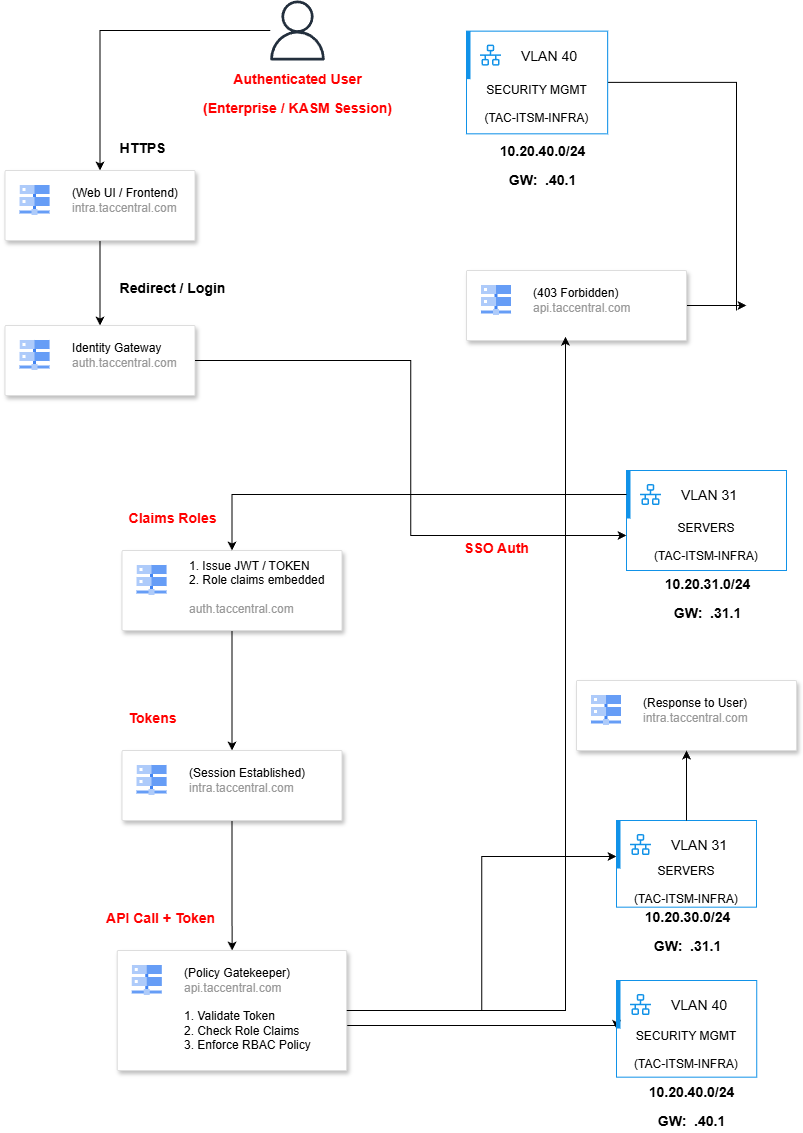
\includegraphics[width=\textwidth]{Images/2zerotrustflow.png}
    \caption{TAC Industries logical network segmentation and infrastructure overview}
    \label{fig:network-architecture}
\end{figure}